% general package(s)
\documentclass[12pt]{article}
\usepackage[margin=0.8in]{geometry}
\usepackage[utf8]{inputenc}
\usepackage[english]{babel}
\usepackage[T1]{fontenc}

% math package(s)
\usepackage{amsmath}
%\usepackage[urw-garamond]{mathdesign}
\usepackage{gensymb}

% figure package(s)
\usepackage{booktabs} % For tables
\usepackage{caption} % For subfigures
\usepackage{float}
\usepackage{graphicx}
\usepackage{listings}
\usepackage{subcaption} % For subfigures
\usepackage{wrapfig} % For inline figures

% reference package(s)
\usepackage[capitalize]{cleveref}

% misc. package(s)
\usepackage{color}

\begin{document}

\title{\makebox[\textwidth][s]{IEA Task 37 on System Engineering in Wind Energy} \\
The Wind Farm Optimization Only Case Study}
\author{Nicholas F. Baker\thanks{Masters Student, Brigham Young University Department of Mechanical Engineering},\  Andrew P. J. Stanley\thanks{Ph.D. Candidate, Brigham Young University Department of Mechanical Engineering}, \ Jared Thomas\thanks{Ph.D. Student, Brigham Young University Department of Mechanical Engineering}, \ and Andrew Ning\thanks{Assistant Professor, Brigham Young University Department of Mechanical Engineering}}
\date{May 2018}

\maketitle{}

\section{Introduction}
   This document defines a simple wind farm layout optimization problem of varying sizes, with the goal of comparing the results obtained when using different optimization methods for a single wake model. While the optimization problem is very simple, we expect the results to assist researchers in understanding the differences that occur due to optimizing wind farms using various numerical methods. The results are expected to serve as a benchmark for future wind farm layout optimization studies. The greater understanding of this simplified problem is expected to aid in solving and interpreting the results of more realistic problems.

\section{Problem Definition}
\subsection{Wind Farm Definition}
There are three (3) wind farm size scenarios which will be optimized:
    \begin{enumerate}
        \item Wind farm of sixteen (16) turbines, boundary radius of 1,500 m.
        \item Wind farm of thirty-six (36) turbines, boundary radius of 2,500 m.
        \item Wind farm of sixty-four (64) turbines, boundary radius of 4,000 m.
    \end{enumerate}
For all wind farm sizes, the wind farm boundary is circular. The specified boundary distance is a radius from the origin.
        %\item The wind turbulence intensity is 0.075.
        %\item Assume the freestream wind speeds given in this document are at hub height. If you need a wind shear, use a power law relationship with a shear exponent of 0.15.

\subsection{Wind Turbine Definition}
    The wind turbine used in this study is the NREL 5MW reference turbine \cite{5MW}. The important parameters are:
    
    \begin{itemize}
        \item \textbf{Rotor Diameter:} 126.4 m
        \item \textbf{Turbine Rating:} 5 MW
        \item \textbf{Cut-In Wind Speed:} 3 m/s
        \item \textbf{Rated Wind Speed:} 11.4 m/s
    \end{itemize}
    
    \noindent The power curve equation is given in \cref{Eq:power} and graphed in \cref{Fig:curve}.
    
    \begin{equation}
        % P(U) = P_{rated}\bigg(\frac{U-V_{cut-in}}{V_{rated}-V_{cut-in}}\bigg)^3
        P(U) = 
            \begin{cases} 
                  0 & U < V_{\textit{cut-in}} \\
                  P_{\textit{rated}}\bigg(\frac{U-V_{\textit{cut-in}}}{V_{\textit{rated}}-V_{\textit{cut-in}}}\bigg)^3 & V_{\textit{cut-in}}\leq U \leq V_{\textit{rated}} \\
                  P_{\textit{rated}} & U > V_{\textit{rated}}
            \end{cases}
        \label{Eq:power}
    \end{equation}
    
    \begin{figure}[H]
        \begin{centering}
        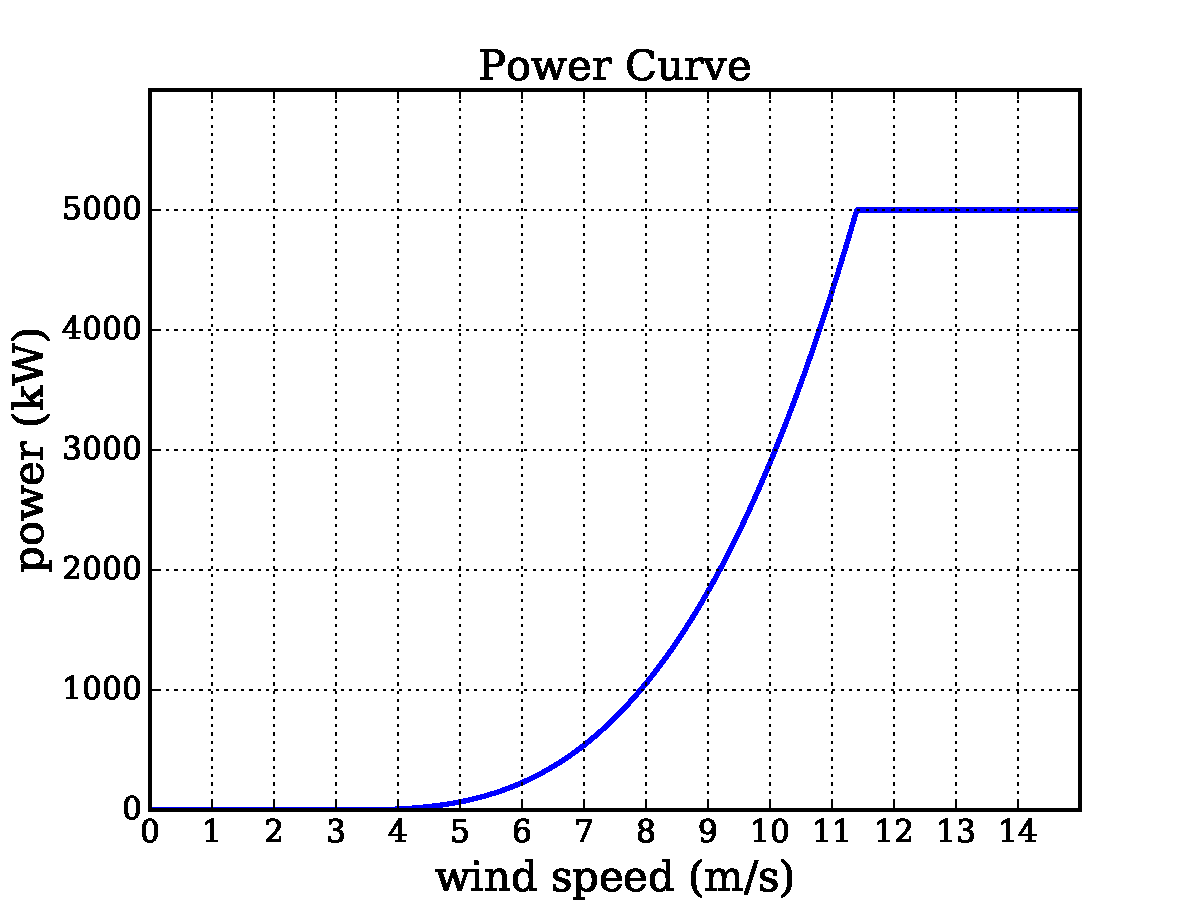
\includegraphics[width=0.75\linewidth]{power_curve.pdf}
        \caption{The wind turbine power curve. \label{Fig:curve}}
        \end{centering}
    \end{figure}

\subsection{Wake Model}
The wake model utilized for this case study is Bastankhah?s Gaussian wake model \cite{Bastankhah2014, Bastankhah2016}. The pertinent files are coded in Python, and are provided alongside this document in a \texttt{.zip} directory.

The governing equation under this model for the velocity deficit in the wake region is:
\begin{equation}
    \frac{\Delta U}{U_{\infty}}
    =
    \Bigg(
        1 - \sqrt{
            1 - \frac{C_T\ \text{cos}\gamma}
                {8\sigma_{y}\sigma_{x}/d^2}
            }
    \Bigg)
            \text{exp}\bigg(
                -0.5\Big(
                    \frac{y-\delta}{\sigma_{y}}
                \Big)^2
            \bigg)
            \text{exp}\bigg(
                -0.5\Big(
                    \frac{z-z_h}{\sigma_{z}}
                \Big)^2
            \bigg)
\end{equation}

Where $\frac{\Delta U}{U_{\infty}}$ is the wake velocity deficit, $C_T$ is the thrust coefficient, and $\gamma$ is the upstream turbine?s yaw angle with respect to the inflow direction (neglected in this study for simplicity). $y-\delta$ and $z-z_h$ are the distances of the point of interest from the wake center in the cross-stream horizontal and vertical directions respectively, and $\sigma_y$ and $\sigma_z$ are the standard deviations of the wake deficit in the cross-stream horizontal and vertical directions as defined in \cref{Eq:SigY,Eq:SigZ}:

\begin{equation}
    \sigma_y = k_y(x - x_0) + \frac{D_r \text{cos}\gamma}{\sqrt{8}} \\
    \label{Eq:SigY}
\end{equation}
\begin{equation}
    \label{Eq:SigZ}
    \sigma_y = k_z(x - x_0) + \frac{D_r}{\sqrt{8}}\\
\end{equation}

In \cref{Eq:SigY,Eq:SigZ}, $x$ is the downstream distance from the turbine generating the wake to the point of interest, $x_0$ is the length of the wake potential core, $D_r$ is the diameter of the turbine generating the wake. $k_y$ and $k_z$ are determined as a function of turbulence intensity ($I$). In this case study, turbulence intensity will also be neglected. Therefore we shall use $k_{y,z} = 0.003678$ \cite{Niayifar2016, Thomas2018}.

\subsection{Wind Speed}
    For this scenario, the freestream wind velocity will be constant throughout the farm, at $13\ m/s$, regardless of turbine location or time of day.

\subsection{Wind Direction Probability}

    For the above specified wind speed, wind direction probability will mimic those found in a geographically linear canyon, using a bi-modal Gaussian distribution. This distribution is defined in  \cref{Eq:freq} and the wind rose is shown below: %in \cref{Fig:freq}.
    
    \begin{equation}
    % PDF = \frac{1}{2\pi\sigma^2}\exp{\Bigg[-\frac{(\theta-\mu)^2}{2\sigma^2}\Bigg]}
        F = w_1\Bigg(\sqrt{\frac{1}{2 \pi \sigma_1^2}}\Bigg)\exp\Bigg(-\frac{(\theta-\mu_1)^2}{2 \sigma_1^2}\Bigg) + w_2\Bigg(\sqrt{\frac{1}{2 \pi \sigma_2^2}}\Bigg)\exp\Bigg(-\frac{(\theta-\mu_2)^2}{2 \sigma_2^2}\Bigg)
    \label{Eq:freq}
    \end{equation}
    %\hspace{-2 cm}
    \begin{minipage}{.65\textwidth}
        \begin{itemize}
            \item \textbf{$\theta$}: wind direction where north is $0 \degree$, measured clockwise.
            \item \textbf{$\mu_1$}: first dominant wind direction ($180\degree$).
            \item \textbf{$\mu_2$}: second dominant wind direction ($350\degree$).
            \item \textbf{$\sigma_1$}: first standard deviation ($20 \degree$).
            \item \textbf{$\sigma_2$}: second standard deviation ($40 \degree$).
            \item \textbf{$w_1$}: first distribution weight ($0.5$).
            \item \textbf{$w_2$}: second distribution weight ($0.5$).
        \end{itemize}
    \end{minipage}
    \begin{minipage}{.4\textwidth}
        \vspace{2 cm}
        \hspace{-2 cm}
            \centering
            \includegraphics[width=\linewidth]{WindRose.eps}
            %\caption{The wind frequency distribution; a bi-modal Gaussian distribution as defined in     \cref{Eq:freq}.
            \label{Fig:freq}
    \end{minipage}
        
\subsection{Code Format}
The relevant code for the above formulas are pre-programmed in Python and released along with this document, in order for each participant to apply their unique optimization methods. The wake model routine takes a specified number of grid locations as inputs, and returns as output the AEP for the given turbine locations.

Though not necessary, alteration to the released AEP calculation code may be done, if required to maximize optimizer effectiveness. Care must be taken, however, that the governing physics equations are not altered to deliver different AEP results. For this reason, base case turbine locations are described in \cref{Sec:RepResults} and corresponding AEP calculations are to be used as validation.

\section{Reporting Results}
\subsection{Submission Contents}\label{Sec:RepResults}
The following information should be included in each submission:

\begin{itemize}
	\item Text file containing your baseline, optimized baseline, initial, and overall optimal computed AEP values in Megawatt-hours, and your optimized baseline, initial and optimal turbine locations in meters. The initial AEP and layout should be from the starting point of your submitted optimized layout. This baseline is designed using a minimum dispersion of 5 rotor diameters between each turbine, in concentric circles. The turbine locations for the baseline value arrangements are given in \Cref{app:BaseGrids}, and are depicted graphically in \cref{fig:BaseLoc}: 

\begin{figure}[H]
\centering
    \hspace*{-2.1 cm}
    \begin{subfigure}{.33\paperwidth}
      \centering
      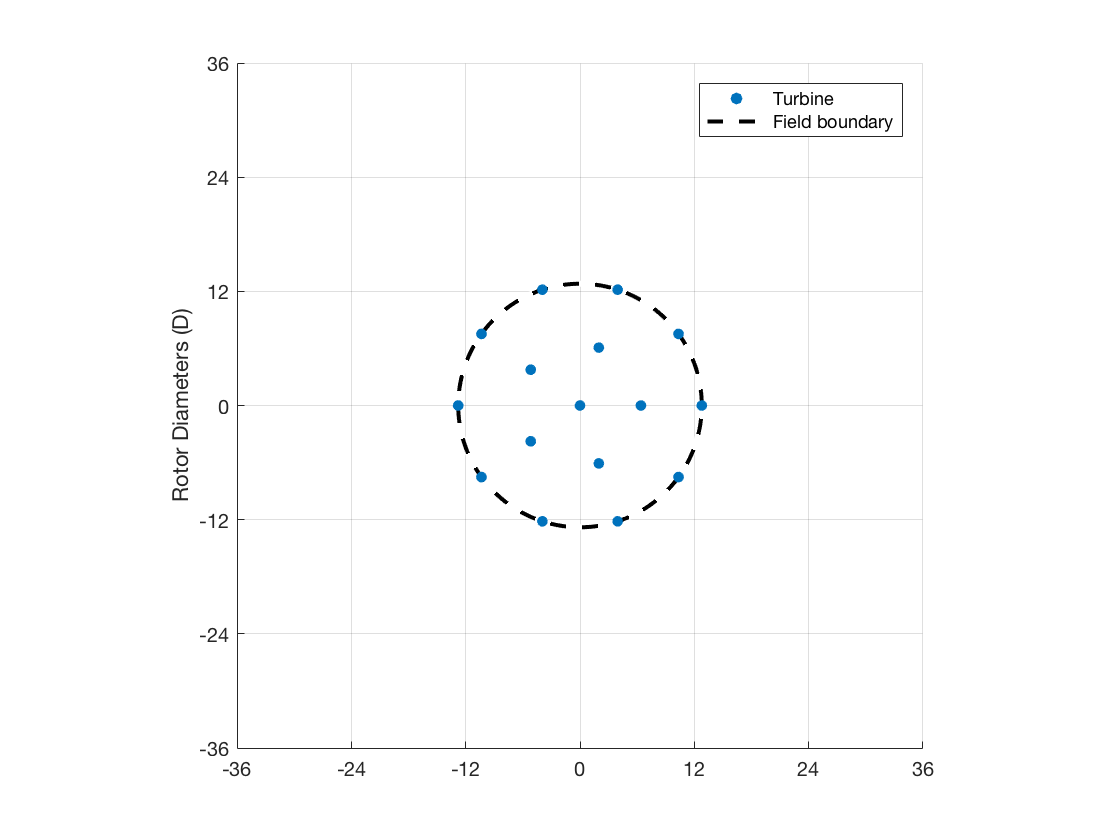
\includegraphics[width=\linewidth]{BaseCase16.png}
      \caption{16 Turbine Farm}
      \label{fig:Base16}
    \end{subfigure}%
    \begin{subfigure}{.33\paperwidth}
      \centering
      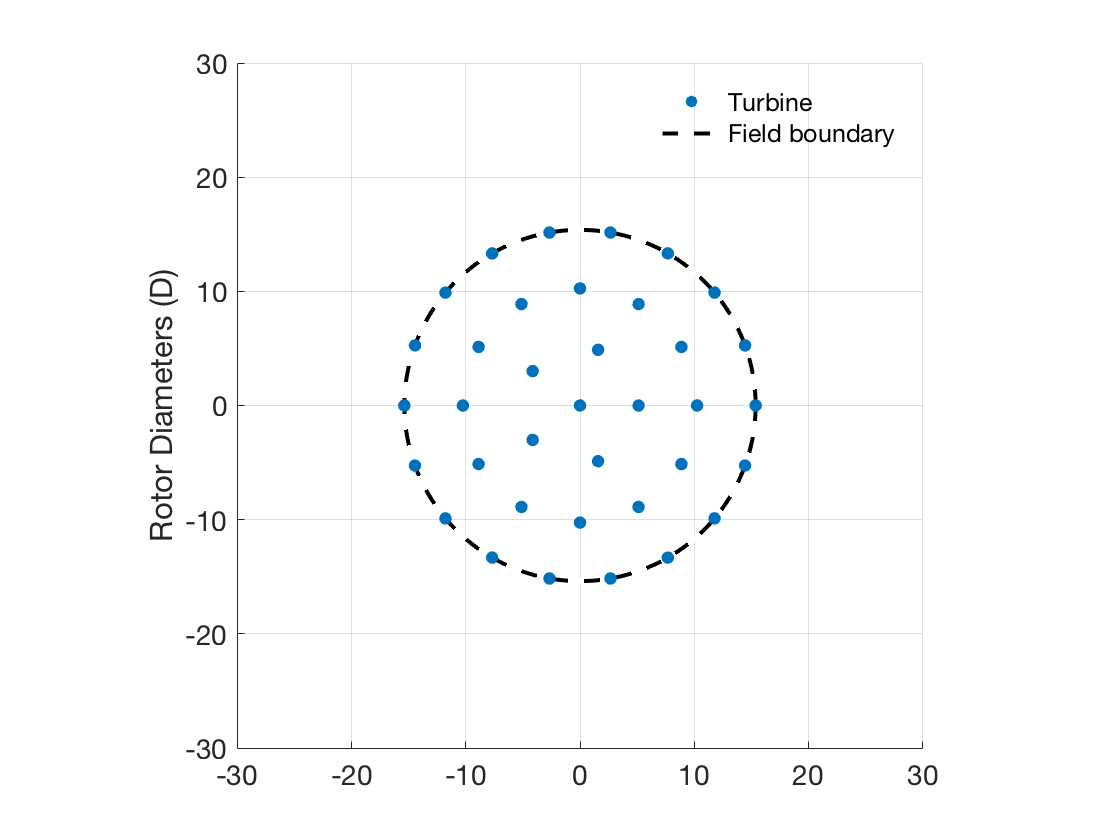
\includegraphics[width=\linewidth]{BaseCase36.png}
      \caption{36 Turbine Farm}
      \label{fig:Base36}
    \end{subfigure}%
    \begin{subfigure}{.33\paperwidth}
      \centering
      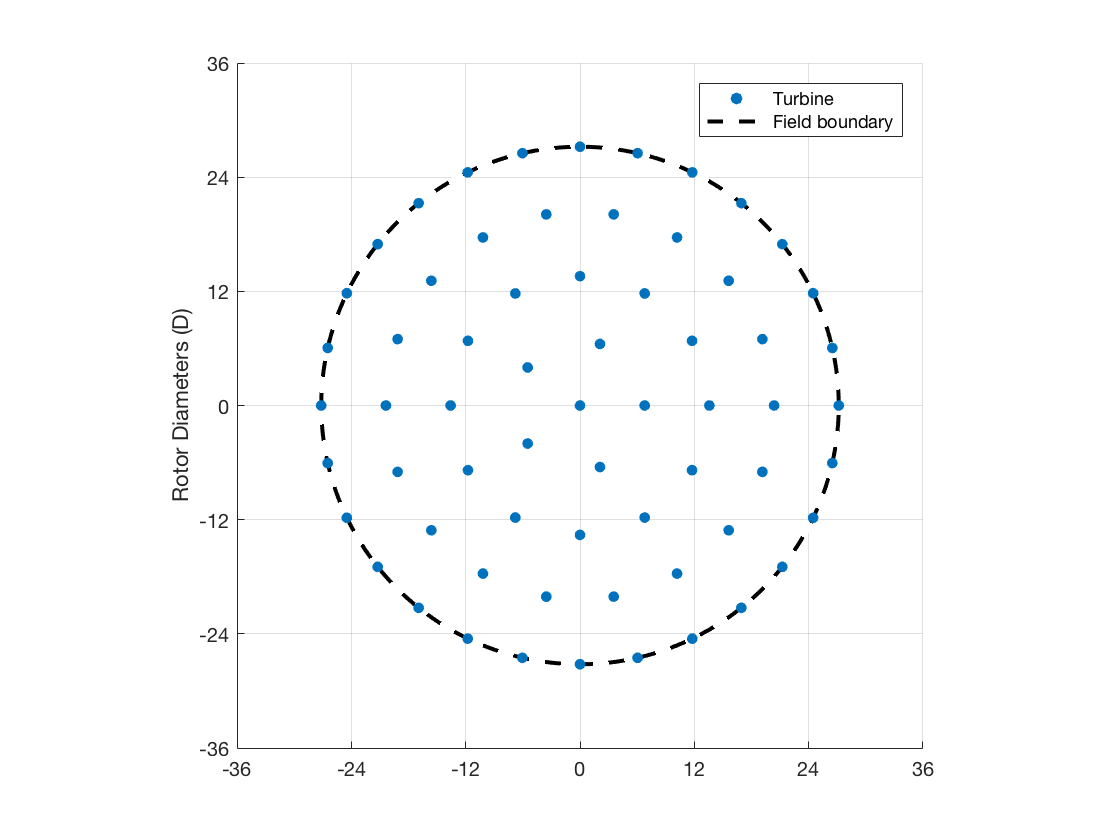
\includegraphics[width=\linewidth]{BaseCase64.png}
      \caption{64 Turbine Farm}
      \label{fig:Base64}
    \end{subfigure}
    \caption{Baseline Turbine Locations}
    \label{fig:BaseLoc}
\end{figure}    

    You are \textbf{NOT} required to start each of your optimizations from these layouts. Feel free to use random starts, intuition, warm starts, or any other selection method for initilizing the turbine locations for your optimizations. Simply report the AEP calculated at these base locations, and a resulting optimized wind farm from a single start using these layouts.
    
	\item Short description containing the relevant details of your method/process. This should include, at a minimum:
    \begin{itemize}
        \item Optimization algorithm (including version and any non-default settings or modifications)
        \begin{itemize}
        	\item Name of algorithm
            \item General type of algorithm (e.g. gradient-free, gradient-based)
            \item Specific algorithm type (e.g. particle-swarm, genetic-algorithm, sequential quadratic programming, etc)
            \item If you used a gradient-based method, how did you obtain the gradients.
            \item Programming language(s) utilized
            \item Other relevant algorithm details
        \end{itemize}
        \item Computer hardware specifications
        \begin{itemize}
            \item Manufacturer/Model/Speed of processor
            \item Number of cores utilized
            \item Amount of RAM allocated per core
        \end{itemize}
        \item Your computed initial and final AEP values
        \item Time required for optimization convergence
        \item Modificiations made (if any) to the original wake model code
        \item Links to relevant code(s) (if possible)
        \item Other details you consider relevant
        \item Bibliography
    \end{itemize}
\end{itemize}
\subsection{Submission Format}
    All submission materials should be submitted in a single compressed \texttt{.zip} directory. The directory should contain:
    
    \begin{enumerate}
        \item A \texttt{.pdf} of the method/process description as described in \cref{Sec:RepResults}
        \item Three (3) \texttt{.txt} files with the quantitative optimization results, one (1) for each farm size, in the following format:
    \end{enumerate}

    The text file for a given farm size should contain two sections: 1) for the baseline, optimized baseline, initial, and  optimal AEP values and 2) for the turbine numbers and their corresponding optimized baseline, initial and optimized $x$ and $y$ locations. Entries in each row should be comma separated. All numbers should be in full double precision.  Please see the example provided in \cref{code:locations}.
    
    \begin{figure}[H]
    \centering
    \framebox{\begin{minipage}{.95\textwidth}
    \texttt{\# base AEP (MWh), optimized base AEP, initial AEP (MWh), optimized AEP (MWh)}\newline
    \texttt{AEP\_base, AEP\_base\_opt, AEP\_init, AEP\_opt}\newline
    
    \texttt{\# turb num, x\_base\_opt(m), y\_base\_opt(m), x\_init(m), y\_init(m), x\_opt(m), y\_opt(m)}\newline
    \texttt{0, x0\_base\_opt, y0\_base\_opt, x0\_init, y0\_init, x0\_opt, y0\_opt}\newline
    \texttt{1, x1\_base\_opt, y1\_base\_opt, x1\_init, y1\_init, x1\_opt, y1\_opt}\newline
    \texttt{2, x2\_base\_opt, y2\_base\_opt, x2\_init, y2\_init, x2\_opt, y2\_opt}\newline
    \texttt{3, x3\_base\_opt, y3\_base\_opt, x3\_init, y3\_init, x3\_opt, y3\_opt}\newline
    \texttt{4, x4\_base\_opt, y4\_base\_opt, x4\_init, y4\_init, x4\_opt, y4\_opt}\newline
    \texttt{5, x5\_base\_opt, y5\_base\_opt, x5\_init, y5\_init, x5\_opt, y5\_opt}\newline
    \texttt{6, x6\_base\_opt, y6\_base\_opt, x6\_init, y6\_init, x6\_opt, y6\_opt}\newline
    \texttt{7, x7\_base\_opt, y7\_base\_opt, x7\_init, y7\_init, x7\_opt, y7\_opt}\newline
    \texttt{8, x8\_base\_opt, y8\_base\_opt, x8\_init, y8\_init, x8\_opt, y8\_opt}\newline
    \texttt{\vdots,
            \quad\quad\quad\vdots, 
            \quad\quad\quad\quad\quad\vdots, \quad\quad\quad\quad\vdots,
            \quad\quad\quad\vdots,
            \quad\quad\vdots,
            \quad\quad\quad\vdots}
    \end{minipage}}
    \caption{Optimization results text file example}
    \label{code:locations}
    \end{figure}

\newpage
\appendix
\section{Baseline Grid Coordinates}
\label{app:BaseGrids}
\vspace{-15pt}
\begin{table}[H]
\begin{minipage}[t]{.33\linewidth}
 \label{tab:TurbLoc16}
 \resizebox{.9\linewidth}{!}{%
    \begin{tabular}{@{}|l|r|r|@{}}
    	\hline
    	\multicolumn{3}{|c|}{(16) Turbine Wind Farm}\\
    	\hline
    	\# & x (m) & y (m) \\
    	\hline
    	0 & 0 & 0 \\ 
    	\hline
    	1 & 758.40 & 0 \\ 
    	\hline
        2 & 234.36 & 721.28 \\ 
    	\hline
        3 & -613.56 & 445.78 \\ 
    	\hline
        4 & -613.56 & -445.78 \\ 
    	\hline
        5 & 234.36 & -721.28 \\ 
    	\hline
    	\hline
        6 & 1516.80 & 0 \\ 
    	\hline
        7 & 1227.10 & 891.55 \\ 
    	\hline
        8 & 468.72 & 1442.60 \\ 
    	\hline
        9 & -468.72 & 1442.60 \\
    	\hline
        10 & -1227.10 & 891.55 \\ 
    	\hline
        11 & -1516.80 & 0 \\ 
        \hline
        12 & -1227.10 & -891.55 \\ 
    	\hline
        13 & -468.72 & -1442.60 \\ 
    	\hline
        14 & 468.72 & -1442.60 \\ 
    	\hline
        15 & 1227.10 & -891.55 \\
    	\hline
    \end{tabular}%
}%
\end{minipage}%
\hfill%
\begin{minipage}[t]{.33\linewidth}
  \label{tab:second_table}
 \resizebox{.9\linewidth}{!}{%
 \begin{tabular}{@{}|l|r|r|@{}}
    	\hline
    	\multicolumn{3}{|c|}{(36) Turbine Wind Farm}\\
    	\hline
    	\# & x (m) & y (m) \\
    	\hline
    	\multicolumn{3}{|c|}{1-5 same as (16) Farm}\\
    	\hline
    	\vdots & \vdots & \vdots \\
    	\hline
    	\hline
    	6 & 1516.80 & 0 \\ 
    	\hline
        7 & 1313.60 & 758.40 \\ 
    	\hline
        8 & 758.40 & 1313.60 \\ 
    	\hline
        9 & 0 & 1516.80 \\
    	\hline
        10 & -758.40 & 1313.60 \\ 
    	\hline
        11 & -1313.60 & 758.40 \\ 
        \hline
        12 & -1516.80 & 0 \\ 
    	\hline
        13 & -1313.60 & -758.40 \\
    	\hline
        14 & -758.40 & -1313.60 \\
    	\hline
        15 & 0 & -1516.80 \\
        \hline
        16 & 758.40 & -1313.60 \\
    	\hline
        17 & 1313.60 & -758.40 \\ 
    	\hline
    	\hline
        18 & 2275.20 & 0 \\ 
    	\hline
        19 & 2138.00 & 778.16 \\ 
    	\hline
        20 & 1742.90 & 1462.50 \\
        \hline
        21 & 1137.60 & 1970.40 \\ 
        \hline
        22 & 395.08 & 2240.60 \\ 
    	\hline
        23 & -395.08 & 2240.60 \\ 
    	\hline
        24 & -1137.60 & 1970.40 \\ 
    	\hline
        25 & -1742.90 & 1462.50 \\ 
    	\hline
        26 & -2138.00 & 778.16 \\ 
    	\hline
        27 & -2275.20 & 0 \\ 
    	\hline
        28 & -2138.00 & -778.16 \\ 
    	\hline
        29 & -1742.90 & -1462.50 \\ 
    	\hline
        30 & -1137.60 & -1970.40 \\ 
        \hline
        31 & -395.08 & -2240.60 \\ 
        \hline
        32 & 395.08 & -2240.60 \\ 
    	\hline
        33 & 1137.60 & -1970.40 \\ 
    	\hline
        34 & 1742.90 & -1462.50 \\ 
    	\hline
        35 & 2138.00 & -778.60 \\ 
    	\hline
    \end{tabular}%
  }%
\end{minipage}%
\hfill%
\begin{minipage}[t]{.33\linewidth}
 \label{tab:third_table}
 \resizebox{.9\linewidth}{!}{%
  \begin{tabular}{@{}|l|r|r|@{}}
    	\hline
    	\multicolumn{3}{|c|}{(64) Turbine Wind Farm}\\
    	\hline
    	\# & x (m) & y (m) \\
    	\hline
    	\multicolumn{3}{|c|}{1-35 same as (36) Farm}\\
    	\hline
    	\vdots & \vdots & \vdots \\ 
    	\hline
    	\hline
        36 & 3033.60 & 0 \\ 
    	\hline
        37 & 2938.30 & 754.43 \\ 
    	\hline
        38 & 2658.40 & 1461.40 \\ 
    	\hline
        39 & 2211.40 & 2076.60 \\ 
    	\hline
        40 & 1625.50 & 2561.40 \\ 
    	\hline
        41 & 937.43 & 2885.10 \\ 
        \hline
        42 & 190.48 & 3027.60 \\ 
    	\hline
        43 & -568.44 & 2979.90 \\ 
    	\hline
        44 & -1291.60 & 2744.90 \\ 
    	\hline
        45 & -1933.70 & 2337.40 \\ 
    	\hline
        46 & -2454.20 & 1783.10 \\ 
    	\hline
        47 & -2820.60 & 1116.70 \\ 
    	\hline
        48 & -3009.70 & 380.21 \\ 
    	\hline
        49 & -3009.70 & -380.21 \\ 
    	\hline
        50 & -2820.60 & -1116.70 \\
        \hline
        51 & -2454.20 & -1783.10 \\ 
        \hline
        52 & -1933.70 & -2337.40 \\ 
    	\hline
        53 & -1291.60 & -2744.90 \\ 
    	\hline
        54 & -568.44 & -2979.90 \\ 
    	\hline
        55 & 190.48 & -3027.60 \\ 
    	\hline
        56 & 937.43 & -2885.10 \\ 
    	\hline
        57 & 1625.50 & -2561.40 \\ 
    	\hline
        58 & 2211.40 & -2076.60 \\ 
    	\hline
        59 & 2658.40 & -1461.40 \\ 
    	\hline
        60 & 2938.30 & -754.43 \\ 
        \hline
        \hline
        61 & 3792.00 & 0 \\ 
        \hline
        62 & -1896.00 & 3284.00 \\ 
    	\hline
    	63 & -1896.00 & -3284.00 \\ 
    	\hline
    \end{tabular}%
 }%
\end{minipage} 
\end{table}

\newpage
\section*{}
\bibliographystyle{unsrt}
\bibliography{references}
\end{document}